\documentclass[10pt,a4paper]{scrartcl}
\usepackage[utf8]{inputenc}
\usepackage[english]{babel}
\usepackage{xcolor}
\usepackage[pdftex]{graphicx}
\usepackage{natbib}
\usepackage{hyperref}
\usepackage{longtable}
\usepackage{array}
\usepackage{enumitem}

\title{Study on the Club of Rome's World3 Model}
\subtitle{Project Introduction to Computational Science 2014\\
University of Amsterdam}
\author{Marc Went, student number 10905847\\Ferry Avis, student number 10904581}

\begin{document}

\maketitle

\section*{Introduction}

This report describes the modelling and simulation project for the course Introduction to Computational Science of the college year 2014-2015 at the University of Amsterdam. The aim of the project is to perform a science project, which will be supported by a simulation study.

We will investigate the Club of Rome's World3 model, which models interactions between industrial growth, population, food production and pollution on a global scale. 

\section*{Background of the model and its use}

In 1968, a group of people from politics, business and science came together to \emph{"discuss the dilemma of prevailing short-term thinking in international affairs and, in particular, the concerns regarding unlimited resource consumption in an increasingly interdependent world"}. This group was named \emph{The Club of Rome}, after the location of the meeting. The first and subsequent meetings resulted in the book `\emph{Limits to Growth}', published in 1972. In the book it was predicted that economic growth could not continue indefinitely, mainly because of the limited availability of natural resources and emissions. Somewhere in the twenty-first century, the growth would end in a uncontrolled decline in population and human welfare.

The model used in the study is called the World3 model. It was the first model that used computer simulation to model the interactions of five submodels, which represent capital, natural resources, agriculture, population and pollution, on a global scale.

The World3 model is far from perfect and was merely a first step in modelling the global world. The authors point out the use of inadequate data, the usage of quantifications of factors for which the influence is not fully clear, such as pollution, and unknown development of technology in the future. Also, natural resources are seen as one identity, while in reality substitutions of depleted natural resources are possible. Increasing prices because of scarcity and the stabilising working of the law of supply and demand are missing in the World3 model; very different from assumptions economists often make in their models.

Despite its flaws, the World3 model is suitable to illustrate the validity of the Club of Rome's hypotheses. The model is an example that it is not necessary to have a perfect model to give an clear insight in problems. The model does not give a prediction, but is sketching alternative scenario's for humanity. For taking appropriate measures to prevent a scenario becoming true, the model and its validity need to be studied and improved extensively. Nevertheless, the authors use the model ``\emph{to identify the future policies that may lead to a stable rather than an unstable behaviour mode}''. The World3 model shows what possibly can go wrong. \cite{vermeulen1976parameter} conclude that, while in \emph{Limits to Growth} very severe measures are suggested for every subsector of the world model in order to avoid the catastrophic population collapse of the standard run, that by combining three changes of 10\% each in the parameters ICOR, FIOAC, ALIC, the collapse of population can also be avoided. They speculate that the real world has so many variables and is so flexible that the correct small pressures on the correct parameters could cause desirable outcomes for the world's evolution.

Limits to Growth received a large amount of publicity at publication. Concerned governments nevertheless continued to go everything they could to stimulate economic growth and no start was made for a transition to a sustainable growth. This was mainly to reduce unemployment. \cite{voorbijdegrenzen} believes that the main contribution of the report is that it led to a continued interest in future of humanity and the start of many discussions.

The difficulty of the problem is that no single country is responsible on its own or able to take appropriate actions. Measures on a world wide scale are necessary, which are very difficult to coordinate. The history of the ozone hole and acid rain shows that global coordination is not impossible. In this report, we will not elaborate on the subject of international cooperation.

\subsubsection*{Critics on the World3 model and Limits to Growth}

The report and the model have received many critics. However, the conclusion remains strong: unlimited growth cannot continue. Some people argued that the equation $y(t) = ae^{rt}$ is also sufficient to show that sustainable growth cannot continue and that the model thus overcomplicates. Others criticize the model for its oversimplification in the aggregation of variables.

Economists often point out that the used assumptions in the models are very different from the axiom's economists often use. Also, the tone of the report is pessimistic. The Club of Rome was wrongfully called the zero growth movement, although the conclusion of the report does not to deny this qualification. In the report there is a dedicated chapter about the conditions to obtain sustainable growth and what growth in a global equilibrium means. Within these conditions, company's can rise and fall, local population can grow and decline. Technological developments can improve the average standard of living.

\section*{Standard run of the model}

Figure \ref{standard-run} shows the behaviour of the standard model, i.e. of the model when no changes to the standard parameters are made.

\begin{figure}
\centering
\begin{minipage}{0.79\textwidth}
\includegraphics[width=\textwidth]{./plaatjes/standard-run.png}
\end{minipage}
\begin{minipage}{0.2\textwidth}
\textcolor[HTML]{e07154}{population}\\
\textcolor[HTML]{b0875e}{resources}\\
\textcolor[HTML]{a8c3a5}{food per capita}\\
\textcolor[HTML]{4a6892}{industrial output per capita}\\
%\textcolor[HTML]{4a8a91}{service output}\\
\textcolor[HTML]{a25563}{pollution index}\\
\textcolor[HTML]{666666}{life expectancy}\\
%\textcolor[HTML]{F6F648}{birth rate}\\
%\textcolor[HTML]{650d99}{death rate}\\
%\textcolor[HTML]{513210}{arable land}\\
%\textcolor[HTML]{185103}{land yield}\\
\end{minipage}
\caption{Behaviour of the model in the standard run}
\label{standard-run}
\end{figure}

Note that the scale on the y-axis is missing. This is because the model does not give predictions, but a direction. The numbers are very likely to be inaccurate and are thus not of great importance.

The model shown in figure \ref{standard-run} shows that around 2040 society will collapse. This happens shortly after the industrial output drops. This manifestation of these catastrophes is an indication that not only the resources are depleted but also the pollution of this world is rising to a record high.

The rising pollution also has a big effect on the life expectancy of the population. Figure 1 shows a correlation around 2045, where pollution is at the largest peak and the life expectancy drops rapidly. Since the turn of a rising life expectancy to a dropping one, the population growth has stagnated, which results in a decay of the human population.

\section*{Research questions}

A full analysis of the parameters of model, the influences of the submodels and making simplifications is enough to write a PhD thesis: see \cite{thissen1978investigations}. However, we would like to study small parts of the model. Based on our own interests and the discussion of the model in Limits to Growth, \cite{thissen1978investigations} and \cite{vermeulen1976parameter}, we ask the following questions:

\begin{itemize}
	\item What is the influence of the size of the population on the use of natural resources?
	\item Can the collapse of population indeed be prevented by increasing the variables ICOR (industrial capital-output ratio) and FIOAC (fraction of inputs allocated to consumption) by 10\% and decreasing ALIC (average lifetime of industrial capital) by 10\%?
	\item What is the influence of the amount of available natural resources?
	\item Do the conditions in the Limits to Growth to obtain sustainable growth indeed lead to a sustainable equilibrium?
\end{itemize}

Additionally, we will investigate behaviour of the model we find remarkable while varying parameters.

\section*{Implementation of the model}

The World3 model is an example of a model in the System dynamics formulation, which is based on feedback loops. Figure \ref{world3} An overview of the model and the interactions between the submodels. We included this figure to give an impression of the size of the model, not for details.

\begin{figure}
\centering
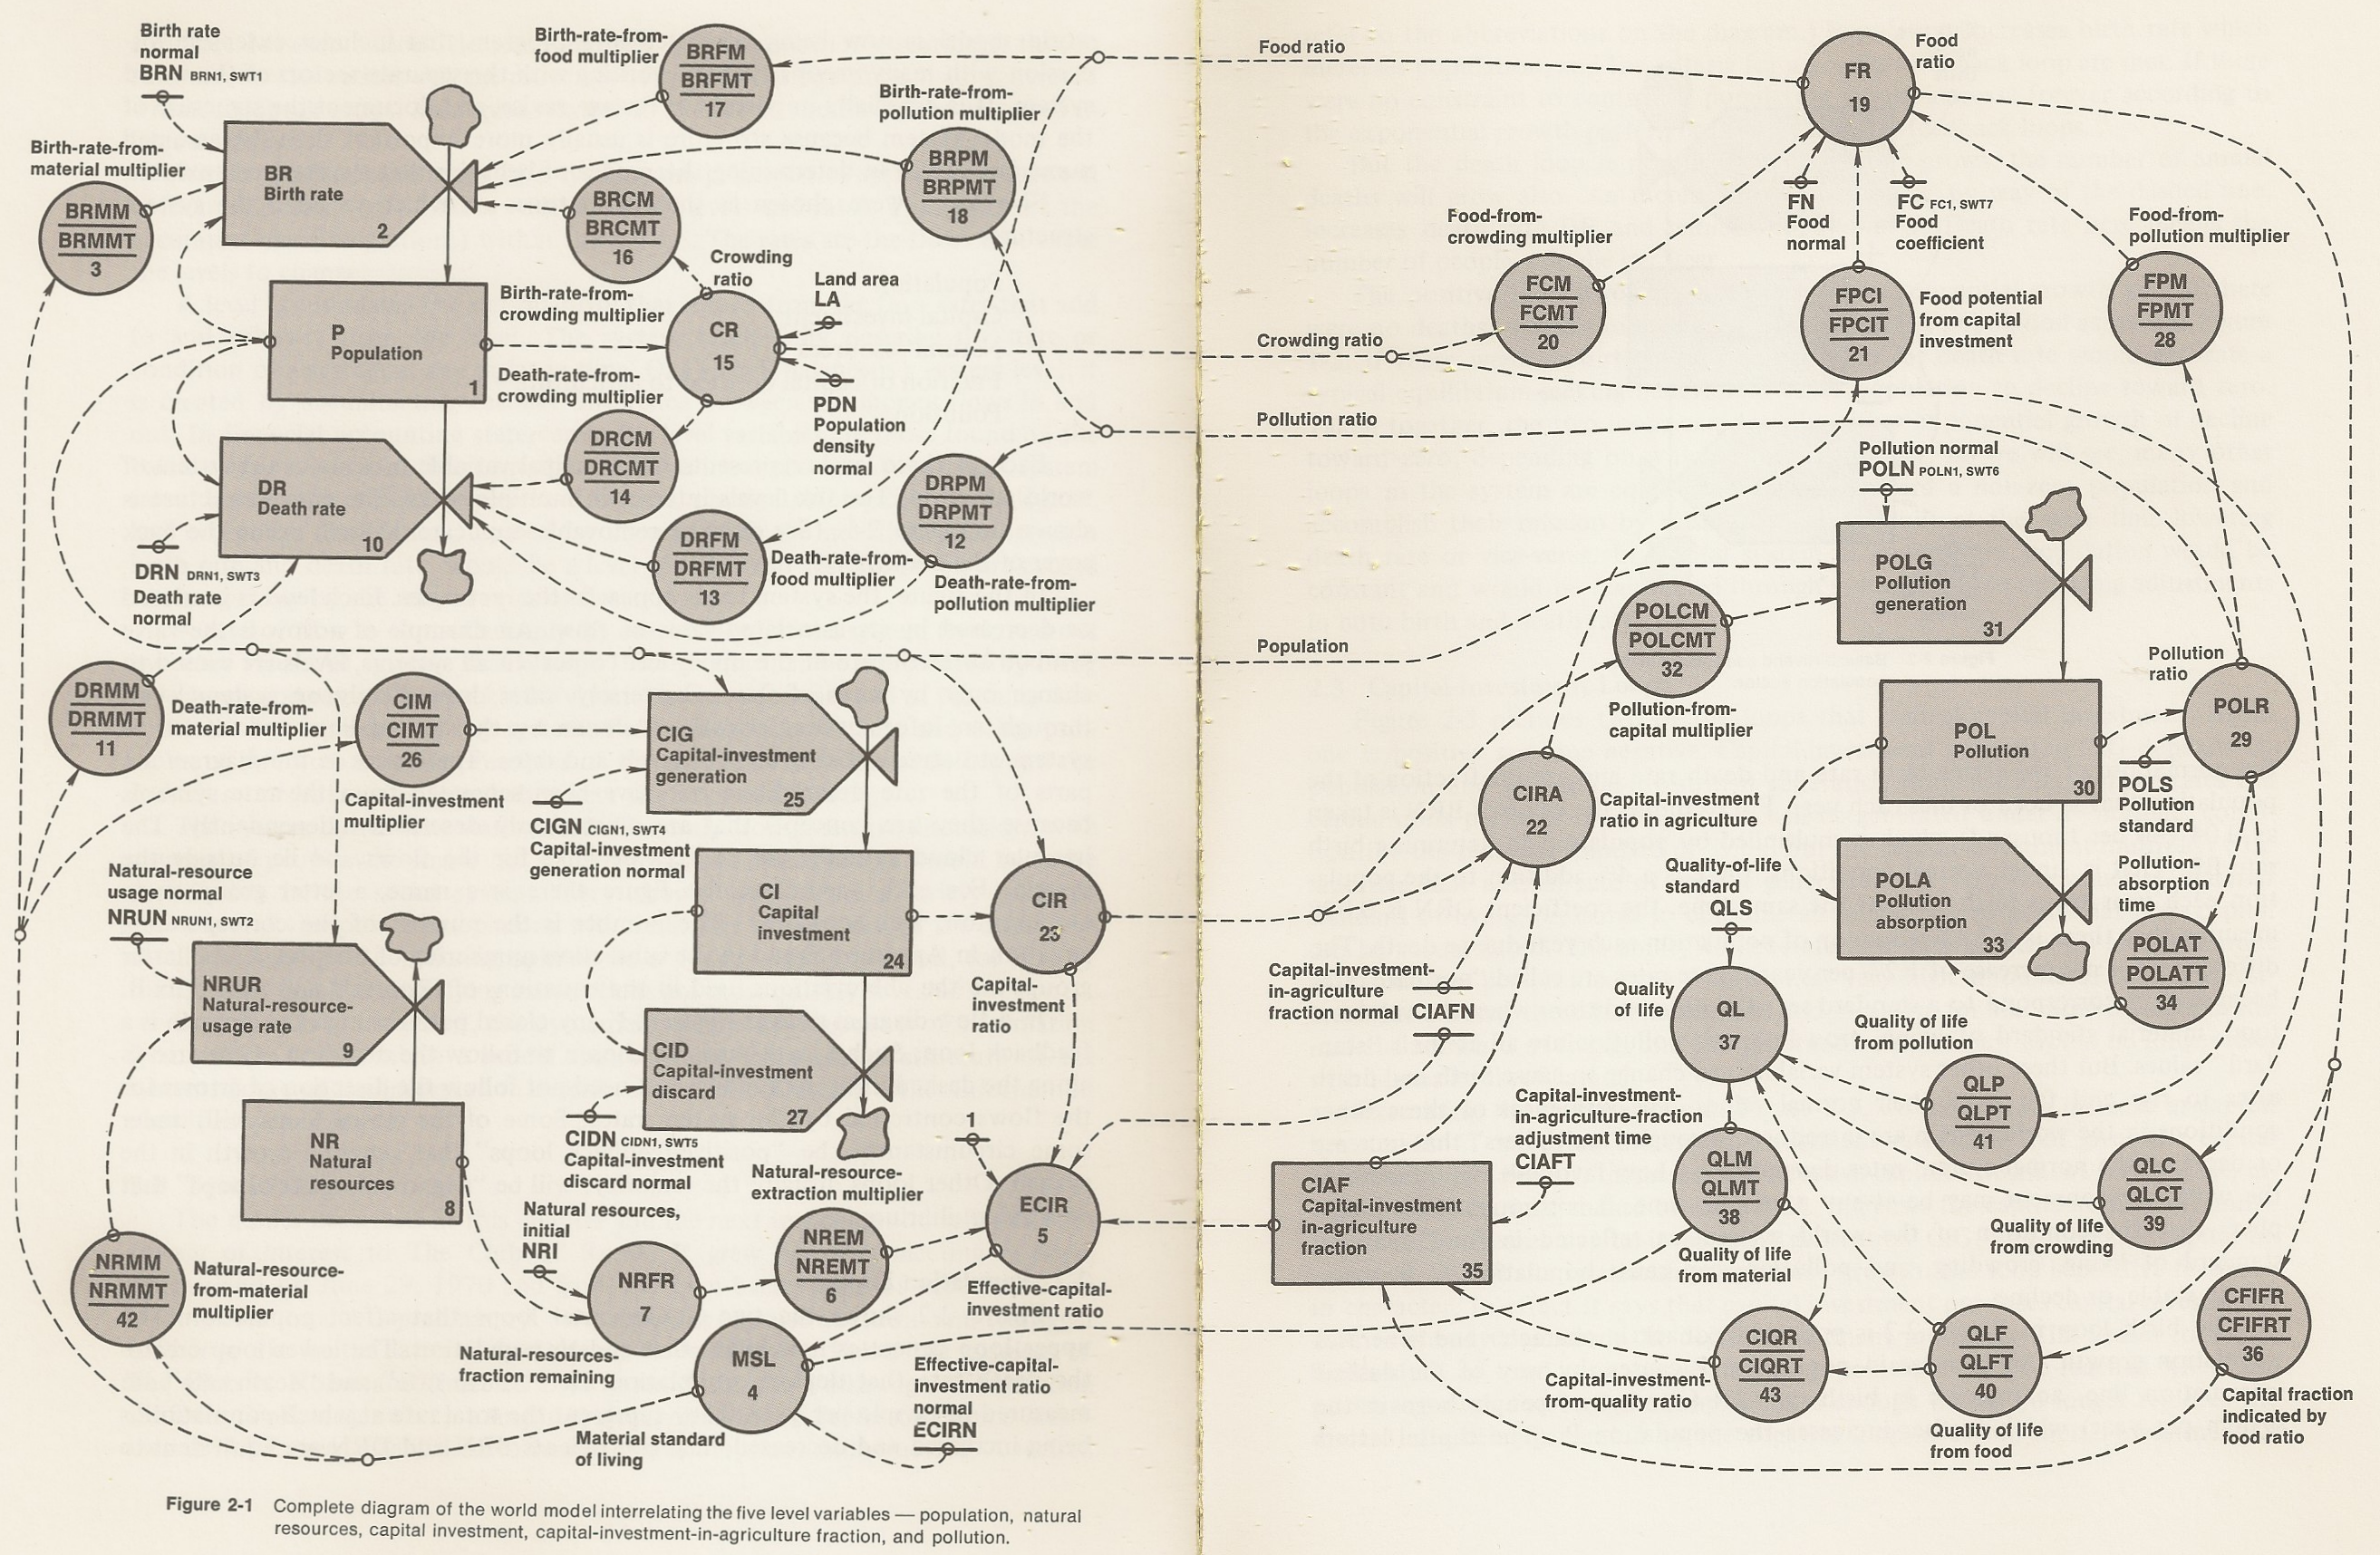
\includegraphics[width=\textwidth]{./plaatjes/model.jpg}
\caption{Diagram of the world model from \cite{forresterworld}}
\label{world3}
\end{figure}

The complete model consists of more than 150 differential equations and variables. The original model is formulated in a special programming language called DYNAMO. The model has since then be ported by the original authors to another language, called STELLA, and extended to include human welfare and footprint indicators. Many others have created ports of the DYNAMO formulation to other languages, such as Java (\url{http://www.world3simulator.org/}), Vensim (\url{http://models.metasd.com/tag/world3/}) and JavaScript (\url{http://bit-player.org/extras/limits/}).

As we wanted to learn how to implement such large model and see how the model really worked, we tried to implement the World3 in the formulation as described in \cite{thissen1978investigations} in Python. In Thissen's formulation, the capital and resource subsectors are merged. However, we did not succeed. First, we will discuss our problems and use one of the ported versions of others for an analysis of the model.

Firstly, we implemented a simplified capital model. \cite{thissen1978investigations} suggested that differences in neither population, agriculture or pollution has any major effect on the capital. This simplified model therefore uses constants for input of these submodels as an alternative.

As we thought this model was too easy we started to replace this simplified capital model with the extended capital model. This model relies on the three other submodels – population, agriculture and pollution. These were also implemented. The interactions between these submodels can be seen in figure \ref{interactions}. He omitted the job sector from World3, as this model proved to influence the model behaviour only under a few, very specific circumstances.

\begin{figure}
\centering
\includegraphics[width=0.5\textwidth]{./plaatjes/submodel-interactions.png}
\caption{Interactions between the four submodels
of World3, without job sector (\cite{thissen1978investigations})}
\label{interactions}
\end{figure}

\subsection*{Simplified resource and capital model}

We were able to implement the simplified resource and capital model from \cite{thissen1978investigations} without problems. This model will be discussed in the results section.

\subsection*{Implementation of Will Thissen's full formulation}

As will be shown in the results section, our implementation of Will Thissen's model does not give correct results.

A particular problem we encountered at the implementation is the use of a function from DYNAMO called DELAY3. This function represents a third-order linear delay. Although this function is implemented in and documented for Vensim, we were not able to find an explanation we could understand.

To come up with a working model, we probably need to understand and implement the original model formulation from \cite{forresterworld} instead of the formulation from \cite{thissen1978investigations}. DYNAMO is an old language, with the special feature that equations can be written down in any order. The compiler does reorder the equations automatically. We expect this to be very challenging to implement this in a sequential language as Python.  After implementing the model in the sequential way, we discovered that the author of the JavaScript port also failed at implementing the model sequentially (\cite{blogpost}). Eventually, he mimicked the automatic ordering of equations of the DYNAMO compiler in JavaScript. Although his source code can be studied, we are not fluent in JavaScript enough to understand his methods.

Unfortunately, we do not have access to the newer STELLA formulation.

\subsubsection*{Approaches taken to find the mistake}

First, the model was thoroughly checked for typing errors. We corrected two or three, but this didn't lead to a working model.

Secondly, different interpretations for the DELAY3 function were implemented. As we think this function represents some kind of moving average, it is our hypothesis that replacing shouldn't have a large impact on the model. This didn't improve our models.

Thirdly, we modified the JavaScript port \cite{blogpost} to print the dependent variables for each submodel from figure \ref{interactions} to study the differences in the change of variables after one iteration. In the first iteration, the submodels only depend on the initial values, of which we assume implemented them correctly. If only one of these values would be wrong, this would be due a mistake in the specific submodel of the variable. However, as can be seen in table \ref{value-differences}, all variables differ. This leaves us clueless.

After one iteration the numbers in the JavaScript version differ in several orders of magnitude from the initial values, which are directly copied from the JavaScript source. Our values seem more probable, but our model is wrong and the JavaScript model isn't. Again, this could be due our unfamiliarity with the JavaScript code, but printing is done by provided functions of the code.

\begin{table}
\centering
\begin{longtable}{|m{1.3cm}|m{3cm}|m{1.2cm}|c|c|m{2cm}|}
\hline
\textbf{Variable} & \textbf{Meaning} & \textbf{Initial value} & \textbf{Python} & \textbf{JavaScript} & \textbf{Units}\\
\hline
POP & Population & 1.6e10 & 1.56e10 & 2.32e10 & amount\\
\hline
IO & Industrial output & 7.90e11 & 6.65e11 & 1.00e-3 & dollars per person-year\\
\hline
SO & Service output & 1.00e13 & 1.00e13 & 0.215 & dollars per year\\
\hline
F & Food & - & 1.72e12 & 7.48e12 & kilograms per year\\
\hline
FIOAA & Fraction of industrial output allocated to agriculture & - & 0.247 & 0.040 & -\\
\hline
AI & Agricultural inputs & - & 7.63e16 & 3.99e-6 & dollars per year\\
\hline
FALM & Fraction of inputs allocated to land maintenance & 0 & 0.040 & 0.052 & -\\
\hline
PPOLX & Index of persistent pollution & 1.36e8 (in 1970) & 0.184 & 7.69e-16 & dimensionless\\
\hline
\end{longtable}
\caption{Values of inter-submodel variables in the standard model after one time step, with $dt$ = 0.5}
\label{value-differences}
\end{table}

\section*{Results and analysis}

\begin{itemize}
	\item What is the influence of the size of the population on the use of natural resources?
	\item Can the collapse of population indeed be prevented by increasing the variables ICOR (industrial capital-output ratio) and FIOAC (fraction of inputs allocated to consumption) by 10\% and decreasing ALIC (average lifetime of industrial capital) by 10\%?
	\item What is the influence of the amount of available natural resources?
	\item Do the conditions in the Limits to Growth to obtain sustainable growth indeed lead to a sustainable equilibrium?
	\item What causes the drastic increase of life expectancy around the Second World War?
\end{itemize}

\subsection*{Simplified capital and resources model}

As stated earlier, this model uses constant input for population, agriculture and pollution on the whole time horizon from 1900 until 2100. When compared to figure \ref{standard-run}, the model seems to be a proper approximation of the population prediction with the original World3 model.

\subsection*{Our Python implementation}

\textcolor{red}{Picture of the standard run in the simplified model and differences with the standard standard run}

\subsection*{JavaScript model}

To answer the research questions posed earlier, we modified the JavaScript port from \cite{blogpost}. The author warns that there are several more versatile and more trustworthy implementations available. Regardless, we decided to use only the JavaScript port due unavailability of source code or complete unfamiliarity with the used programming languages of other models.

\begin{figure}
\centering
\begin{minipage}{0.79\textwidth}
\includegraphics[width=\textwidth]{./plaatjes/multiplier-2.png}
\end{minipage}
\begin{minipage}{0.2\textwidth}
\textcolor[HTML]{e07154}{population}\\
\textcolor[HTML]{b0875e}{resources}\\
\textcolor[HTML]{a8c3a5}{food per capita}\\
\textcolor[HTML]{4a6892}{industrial output per capita}\\
%\textcolor[HTML]{4a8a91}{service output}\\
\textcolor[HTML]{a25563}{pollution index}\\
\textcolor[HTML]{666666}{life expectancy}\\
%\textcolor[HTML]{F6F648}{birth rate}\\
%\textcolor[HTML]{650d99}{death rate}\\
%\textcolor[HTML]{513210}{arable land}\\
%\textcolor[HTML]{185103}{land yield}\\
\end{minipage}
\caption{Behaviour of the model with twice the amount of available non renewable resources}
\label{resources-2}
\end{figure}

When figure \ref{resources-2} is compared to figure \ref{standard-run}, it can be seen that the decrease of the population is delayed when natural resources are increased. Industrial output attains a higher maximum and pollution rises drastically. One of the examples of the use of incorrect data was the amount of available natural resources. New techniques have made it, for example, possible to extract oil deeper from the earth. However, as we will see, this has no influence on the main conclusion of the report.

Figure \ref{composition} is a composition of several figures. First, it is shown that when the fraction of output consumed is lowered from the standard 0.43 to 0.01, industrial output grows enormously fast and population declines around 1960 because of pollution. the second picture of the compilation displays the behaviour of the model when the time step is changed to 2. This reminds us of the unstability of the discrete Lotka Volterra model in the lectures.

The second two pictures in figure \ref{composition} display the behaviour with the fraction of consumed output 0.51 and 0.52. Changing this parameter by such small amount causes a major difference in. Unfortunately, the model doesn't support the human welfare index of newer versions of the World3 model. Finally, 

\begin{figure}
\centering
\begin{minipage}{0.49\textwidth}
\includegraphics[width=\textwidth]{./plaatjes/output-consumed-0,01.png}
\end{minipage}
\begin{minipage}{0.49\textwidth}
\includegraphics[width=\textwidth]{./plaatjes/timestep-2.png}
\end{minipage}
\begin{minipage}{0.49\textwidth}
\includegraphics[width=\textwidth]{./plaatjes/output-consumed-0,51.png}
\end{minipage}
\begin{minipage}{0.49\textwidth}
\includegraphics[width=\textwidth]{./plaatjes/output-consumed-0,52.png}
\end{minipage}
\caption{Left to right, upper to lower: standard run with the fraction of output consumed 0.01, standard run with $dt=2$, standard run with fraction of output 0.51 and standard run with fraction of output 0.52}
\label{composition}
\end{figure}

To investigate the phenomenon that caused the drastic increase in life expectancy around the Second World War, we printed the values of the life expectancy and the components it is computed from in time. It appeared that in 1940 the life time multiplier from health services increased. The code showed a hard coded policy change in this year, so we went on to investigate why. In \cite{meadows1974dynamics} it is described that the advances in technology caused a major increase in life expectancy from 1900 until 1966. It was chosen to implement this by a simple shift from the postulated 1900 table function to the 1966 in 1940. We did not notice this at implementing the Python model, as Thissen does not make this distinction. 

\section*{The Club of Rome today}

Today, the Club of Rome still exists. The focus in its early years was on the nature of the global problems and on new pathways for world development. Currently, the Club of Rome defines and communicates the elements of a new economy, which produces real wealth and well-being, without degrading natural resources and and with providing meaningful jobs and sufficient income for all people.

\section*{Conclusion}

The World3 model and Limits to Growth discusses interesting and urgent problems. A full analysis of the model has proven to be enough work for a PhD thesis, i.e. more time than we have for this assignment. We haven't succeed to implement the World3 model in Python.

As for which ``dynamic tendencies'', as it is called in the Limits of Growth, will indicate how the future is going to be, is not yet clear. We are currently at the peak of welfare predicted by the model. Some scientists are optimistic about the ability to deal with the issues before the world collapses, while others are not. The consequences of an overshoot are already observable, such as in global warming.

\bibliographystyle{abbrvnat}
\nocite{*}
\bibliography{bibliografie}

\end{document}